\documentclass{book}

\usepackage{cmap}

\usepackage[russian,english]{babel}
\usepackage[T2A]{fontenc}
\usepackage[default]{sourcesanspro}

\usepackage{ifthen}

\usepackage{listings}
\usepackage{url}
\usepackage[cm]{fullpage}
\usepackage{graphicx}
\usepackage{framed}
\usepackage{color}
\usepackage{float}
\usepackage{tikz}
\usetikzlibrary{arrows}
\usepackage[nottoc]{tocbibind}
%\usepackage{esint}
%\usepackage{charter}
%\usepackage[charter]{mathdesign}
\usepackage[footnote,printonlyused,withpage]{acronym}
\usepackage[]{hyperref} % should be last

\definecolor{lstbgcolor}{rgb}{0.94,0.94,0.94}

\newcommand{\TT}[1]{\texttt{#1}}

\newcommand{\TITLE}{Math-notes}
\newcommand{\AUTHOR}{Dennis Yurichev \TT{<dennis(@)yurichev.com>}}

\hypersetup{
    pdftex,
    colorlinks=true,
    allcolors=blue,
    pdfauthor={\AUTHOR},
    pdftitle={\TITLE},
    pdfpagemode=None
}

\lstset{
    backgroundcolor=\color{lstbgcolor},
    basicstyle=\ttfamily, 
    breaklines=true,
    frame=single,
    columns=fullflexible,keepspaces,
}

\author{\AUTHOR}
\title{\TITLE}
%\date{August-2015 --- ...}

\begin{document}

% reworked from http://tex.stackexchange.com/questions/26181/create-context-sensitive-headings

\newcommand{\currentlevel}{}

\newcommand{\leveldown}%
{   
    \ifthenelse{\equal{\currentlevel}{sp}}%
    {\renewcommand{\currentlevel}{sp}}{}%    
    \ifthenelse{\equal{\currentlevel}{p}}%
    {\renewcommand{\currentlevel}{sp}}{}%    
    \ifthenelse{\equal{\currentlevel}{sss}}%
    {\renewcommand{\currentlevel}{p}}{}%    
    \ifthenelse{\equal{\currentlevel}{ss}}%
    {\renewcommand{\currentlevel}{sss}}{}%    
    \ifthenelse{\equal{\currentlevel}{s}}%
    {\renewcommand{\currentlevel}{ss}}{}%
    \ifthenelse{\equal{\currentlevel}{c}}%
    {\renewcommand{\currentlevel}{s}}{}%
}

\newcommand{\levelup}%
{
    \ifthenelse{\equal{\currentlevel}{c}}%
    {\renewcommand{\currentlevel}{c}}{}%
    \ifthenelse{\equal{\currentlevel}{s}}%
    {\renewcommand{\currentlevel}{c}}{}%
    \ifthenelse{\equal{\currentlevel}{ss}}%
    {\renewcommand{\currentlevel}{s}}{}%
    \ifthenelse{\equal{\currentlevel}{sss}}%
    {\renewcommand{\currentlevel}{ss}}{}
    \ifthenelse{\equal{\currentlevel}{p}}%
    {\renewcommand{\currentlevel}{sss}}{}
    \ifthenelse{\equal{\currentlevel}{sp}}%
    {\renewcommand{\currentlevel}{p}}{}%
}

\newcommand{\myheading}[1]%
{   \ifthenelse{\equal{\currentlevel}{c}}%
    {\chapter{#1}}{}%
    \ifthenelse{\equal{\currentlevel}{s}}%
    {\section{#1}}{}%
    \ifthenelse{\equal{\currentlevel}{ss}}%
    {\subsection{#1}}{}%
    \ifthenelse{\equal{\currentlevel}{sss}}%
    {\subsubsection{#1}}{}%
    \ifthenelse{\equal{\currentlevel}{p}}%
    {\myparagraph{#1}}{}%
    \ifthenelse{\equal{\currentlevel}{sp}}%
    {\mysubparagraph{#1}}{}%
}

\newcommand{\newchapter}[1]{\chapter{#1}\renewcommand{\currentlevel}{c}}
\newcommand{\newsection}[1]{\section{#1}\renewcommand{\currentlevel}{s}}
\newcommand{\newsubection}[1]{\subsection{#1}\renewcommand{\currentlevel}{ss}}
\newcommand{\newsubsubection}[1]{\subsubsection{#1}\renewcommand{\currentlevel}{sss}}
\newcommand{\newparagraph}[1]{\myparagraph{#1}\renewcommand{\currentlevel}{p}}
\newcommand{\newsubparagraph}[1]{\mysubparagraph{#1}\renewcommand{\currentlevel}{sp}}


\maketitle

\tableofcontents

%\section*{Thanks}

%Thanks to those who helped: Slava ``Avid'' Kazakov, Serhiy Matviychuk.

\mainmatter

%\newchapter{Modulo arithmetics}

\leveldown{}

\myheading{Quick introduction into modular arithmetic}

\leveldown{}

Modular arithmetic is an environment where all values are limited by some number (modulo).
Many textbooks has clock as example. Let's imagine old mechanical analog clock.
There hour hand points to one of number in bounds of 0..11 (zero is usually shown as 12).
What hour will be if to sum up 10 hours (no matter, AM or PM) and 4 hours?
10+4 is 14 or 2 by modulo 12.
Naively you can just sum up numbers and subtract modulo base (12) as long as it's possible.

Modern digital watch shows time in 24 hours format, so hour there is a variable in modulo base 24.
But minutes and seconds are in modulo 60 (let's forget about leap seconds for now).

Another example is US imperial system of measurement: human height is measured in feets and inches.
There are 12 inches in feet, so when you sum up some lengths, you increase feet variable each time you've got more than 12 inches.

Another example I would recall is password cracking utilities. Often, characters set is defined in such utilities.
And when you set all Latin characters plus numbers, you've got 26+10=36 characters in total.
If you brute-forcing a 6-characters password, you've got 6 variables, each is limited by 36.
And when you increase last variable, it happens in modular arithmetic rules: if you got 36, set last variable to 0 and increase penultimate
one. If it's also 36, do the same. If the very first variable is 36, then stop.
Modular arithmetic may be very helpful when you write multi-threading (or distributed) password cracking utility and you need to slice all passwords space by even
parts.

\myhrule{}

This is yet another application of modulo arithmetic, which many of us encountered in childhood.

Given a counting rhyme, like:

\begin{lstlisting}
    Eeny, meeny, miny, moe,
    Catch a tiger by the toe.
    If he hollers, let him go,
    Eeny, meeny, miny, moe.
\end{lstlisting}
( \url{https://en.wikipedia.org/wiki/Eeny,_meeny,_miny,_moe} )

... predict, who will be choosen.

If I'm correct, that rhyme has 16 items, and if a group of kids constist of, say, 5 kids, who will be choosen?
16 mod 5 = 1, meaning, the next kid after the one at whom counting had begun.

Or 7 kids, 16 mod 7 = 2. Count two kids after the first one.

If you can calculate this quickly, you can probably get an advantage by choosing a better place within a circle...

\myhrule{}

Now let's recall old mechanical counters which were widespread in pre-digital era:

\begin{figure}[H]
\centering
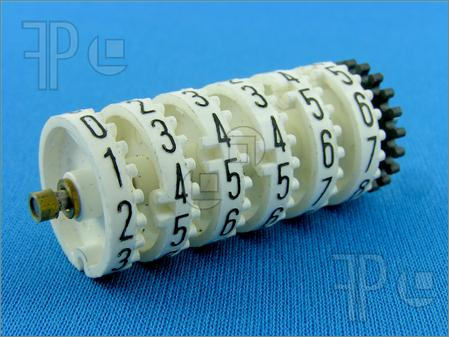
\includegraphics[scale=0.66]{modulo/counter.jpg}
\caption{The picture was stolen from \url{http://www.featurepics.com/} --- sorry for that!}
\end{figure}

This counter has 6 wheels, so it can count from 0 to $10^{6}-1$ or 999999.
When you have 999999 and you increase the counter, it will resetting to 000000---
this situation is usually understood by engineers and computer programmers as overflow.
And if you have 000000 and you decrease it, the counter will show you 999999.
This situation is often called ``wrap around''.
See also: \url{http://en.wikipedia.org/wiki/Integer_overflow}.

\myheading{Modular arithmetic on CPUs}

The reason I talk about mechanical counter is that CPU registers acting in the very same way, because this is, perhaps, simplest possible and efficient way
to compute using integer numbers.

This implies that almost all operations on integer values on your CPU is happens by modulo $2^{32}$ or $2^{64}$ depending on your CPU.
For example, you can sum up 0x87654321 and 0xDEADBABA, which resulting in 0x16612FDDB.
This value is too big for 32-bit register, so only 0x6612FDDB is stored, and leading 1 is dropped.
If you will multiply these two numbers, the actual result it 0x75C5B266EDA5BFFA, which is also too big, so only low 32-bit part is stored into destination
register: 0xEDA5BFFA. This is what happens when you multiply numbers in plain C/C++ language, but some readers may argue:
when sum is too big for register, CF (carry flag) is set, and it can be used after.
And there is x86 MUL instruction which in fact produces 64-bit result in 32-bit environment (in EDX:EAX registers pair).
That's true, but observing just 32-bit registers, this is exactly environment of modulo with base $2^{32}$.

Now that leads to surprising consequence: almost every result of arithmetic operation stored in general purpose register of
32-bit CPU is in fact
remainder of division operation: result is always divided by $2^{32}$ and remainder is left in register.
For example, 0x16612FDDB is too large for storage, and it's divided by $2^{32}$ (or 0x100000000).
The result of division (quotient) is 1 (which is dropped) and remainder is 0x6612FDDB (which is stored as a result).
0x75C5B266EDA5BFFA divided by $2^{32}$ (0x100000000) produces 0x75C5B266 as a result of division (quotient) and 0xEDA5BFFA as a remainder, the latter is stored.

And if your code is 32-bit one in 64-bit environment, CPU registers are bigger, so the whole result can be stored there,
but high half is hidden behind the scenes -- because no 32-bit code can access it.

By the way, this is the reason why remainder calculation is often called "division by modulo".
C/C++ has a percent sign (``\%'') for this operation, but some other PLs like Pascal and Haskell has "mod" operator.

Usually, almost all sane computer programmers works with variables as they never wrapping around and value here is always in some limits which
are defined preliminarily.
However, this implicit division operation or "wrapping around" can be exploited usefully.

\myheading{Remainder of division by modulo $2^{n}$}

... can be easily computed with AND operation.
If you need a random number in range of 0..16, here you go: rand()\&0xF.
That helps sometimes.</p>

<p>For example, you need a some kind of wrapping counter variable which always should be in 0..16 range. What you do?
Programmers often write this:

\begin{lstlisting}[style=customc]
int counter=0;
...
counter++;
if (counter==16)
    counter=0;
\end{lstlisting}

But here is a version without conditional branching:

\begin{lstlisting}[style=customc]
int counter=0;
...
counter++;
counter=counter&0xF;
\end{lstlisting}

As an example, this I found in the git source code:

\begin{lstlisting}[style=customc]
char *sha1_to_hex(const unsigned char *sha1)
{
        static int bufno;
        static char hexbuffer[4][GIT_SHA1_HEXSZ + 1];
        static const char hex[] = "0123456789abcdef";
        char *buffer = hexbuffer[3 & ++bufno], *buf = buffer;
        int i;

        for (i = 0; i < GIT_SHA1_RAWSZ; i++) {
                unsigned int val = *sha1++;
                *buf++ = hex[val >> 4];
                *buf++ = hex[val & 0xf];
        }
        *buf = '\0';

        return buffer;
}
\end{lstlisting}

( \url{https://github.com/git/git/blob/aa1c6fdf478c023180e5ca5f1658b00a72592dc6/hex.c} )

This function returns a pointer to the string containing hexadecimal representation of SHA1 digest \\
(like "4e1243bd22c66e76c2ba9eddc1f91394e57f9f83").
But this is plain C and you can calculate SHA1 for some block, get pointer to the string, then calculate SHA1 for another block, get pointer to the string,
and both pointers are still points to the same string buffer containing the result of the second calculation.
As a solution, it's possible to allocate/deallocate string buffer each time, but more hackish way is to have several buffers (4 are here) and fill the next each time.
The \textit{bufno} variable here is a buffer counter in 0..3 range.
Its value increments each time, and its value is also always
kept in limits
by AND operation (\textit{3 \& ++bufno}).

The author of this piece of code (seemingly Linus Torvalds himself) went even further and forgot (?)
to initialize \textit{bufno} counter variable, which will
have random garbage at the function start.
Indeed: no matter, which buffer we are starting each time!
This can be mistake which isn't affect correctness of the code, or maybe this is left so intentionally -- I don't know.

\myheading{Getting random numbers}

When you write some kind of videogame, you need random numbers, and the standard C/C++ rand() function gives you them in 0..0x7FFF range (MSVC)
or in 0..0x7FFFFFFF range (GCC).
And when you need a random number in 0..10 range, the common way to do it is:

\begin{lstlisting}
X_coord_of_something_spawned_somewhere=rand() % 10;
Y_coord_of_something_spawned_somewhere=rand() % 10;
\end{lstlisting}

No matter what compiler do you use, you can think about it as 10 is subtraced from rand() result, as long as there is still
a number bigger than 10.
Hence, result is remainder of division of rand() result by 10.

One nasty consequence is that neither 0x8000 nor 0x80000000 cannot be divided by 10 evenly, so you'll get some numbers slightly more often than others.

I tried to calculate in Mathematica. Here is what you get if you write <i>rand() % 3</i> and rand() produce numbers in range of 0..0x7FFF (like MSVC):

\begin{lstlisting}
In[]:= Counts[Map[Mod[#, 3] &, Range[0, 16^^8000 - 1]]]
Out[]= <|0 -> 10923, 1 -> 10923, 2 -> 10922|>
\end{lstlisting}

So a number 2 appers slightly seldom than others.

Here is a result for \textit{rand() \% 10}:

\begin{lstlisting}
In[]:= Counts[Map[Mod[#, 10] &, Range[0, 16^^8000 - 1]]]
Out[]= <|0 -> 3277, 1 -> 3277, 2 -> 3277, 3 -> 3277, 4 -> 3277,
 5 -> 3277, 6 -> 3277, 7 -> 3277, 8 -> 3276, 9 -> 3276|>
\end{lstlisting}

Numbers 8 and 9 appears slightly seldom.

Here is a result for \textit{rand() \% 100}:

\begin{lstlisting}
In[]:= Counts[Map[Mod[#, 100] &, Range[0, 16^^8000 - 1]]]
Out[]= <|0 -> 328, 1 -> 328, 2 -> 328, 3 -> 328, 4 -> 328, 5 -> 328,
  6 -> 328, 7 -> 328, 8 -> 328, 9 -> 328, 10 -> 328, 11 -> 328,
 12 -> 328, 13 -> 328, 14 -> 328, 15 -> 328, 16 -> 328, 17 -> 328,
 18 -> 328, 19 -> 328, 20 -> 328, 21 -> 328, 22 -> 328, 23 -> 328,
 24 -> 328, 25 -> 328, 26 -> 328, 27 -> 328, 28 -> 328, 29 -> 328,
 30 -> 328, 31 -> 328, 32 -> 328, 33 -> 328, 34 -> 328, 35 -> 328,
 36 -> 328, 37 -> 328, 38 -> 328, 39 -> 328, 40 -> 328, 41 -> 328,
 42 -> 328, 43 -> 328, 44 -> 328, 45 -> 328, 46 -> 328, 47 -> 328,
 48 -> 328, 49 -> 328, 50 -> 328, 51 -> 328, 52 -> 328, 53 -> 328,
 54 -> 328, 55 -> 328, 56 -> 328, 57 -> 328, 58 -> 328, 59 -> 328,
 60 -> 328, 61 -> 328, 62 -> 328, 63 -> 328, 64 -> 328, 65 -> 328,
 66 -> 328, 67 -> 328, 68 -> 327, 69 -> 327, 70 -> 327, 71 -> 327,
 72 -> 327, 73 -> 327, 74 -> 327, 75 -> 327, 76 -> 327, 77 -> 327,
 78 -> 327, 79 -> 327, 80 -> 327, 81 -> 327, 82 -> 327, 83 -> 327,
 84 -> 327, 85 -> 327, 86 -> 327, 87 -> 327, 88 -> 327, 89 -> 327,
 90 -> 327, 91 -> 327, 92 -> 327, 93 -> 327, 94 -> 327, 95 -> 327,
 96 -> 327, 97 -> 327, 98 -> 327, 99 -> 327|>
\end{lstlisting}

\dots now larger part of numbers happens slightly seldom, these are 68...99.

This is sometimes called \textit{modulo bias}. It's perhaps acceptable for videogames, but may be critical for scientific simulations, including Monte Carlo method.

Constructing a \ac{PRNG} with uniform distribution may be tricky, there are couple of methods:
\url{http://www.reddit.com/r/algorithms/comments/39tire/using_a_01_generator_generate_a_random_number/},
\url{http://www.prismmodelchecker.org/casestudies/dice.php}.

\levelup{}


\myheading{Modulo inverse}

Example: this piece of code divides by 17:

\begin{lstlisting}[style=customc]
#include <stdio.h>
#include <stdint.h>

uint32_t div17 (uint32_t a)
{
	return a*0xf0f0f0f1;
};

int main()
{
	printf ("%d\n", div17(1700));	// result=100
	printf ("%d\n", div17(34));	// result=2
	printf ("%d\n", div17(2091));	// result=123
};
\end{lstlisting}

Unfortunately, it can't produce correct quotient if $remainder \neq 0$, so it's not very useful.
But this code (which divides by 9, though) works correctly in all cases:

\begin{lstlisting}[style=customc]
#include <stdint.h>

uint32_t divide_by_9 (uint32_t a)
{
        return ((uint64_t)a * (uint64_t)954437177) >> 33; // 954437177 = 0x38e38e39
};
\end{lstlisting}

How it works?

\myhrule{}

Let's imagine, we work on 4-bit CPU, it has 4-bit registers, each can hold a value in 0..15 range.

Now we want to divide by 3 using multiplication.
Let's find modulo inverse of 3 using Wolfram Mathematica:

\begin{lstlisting}
In[]:= PowerMod[3, -1, 16]
Out[]= 11
\end{lstlisting}

This is in fact solution of a $3m=16k+1$ equation ($16 = 2^4$):

\begin{lstlisting}
In[]:= FindInstance[3 m == 16 k + 1, {m, k}, Integers]
Out[]= {{m -> 11, k -> 2}}
\end{lstlisting}

The "magic number" for division by 3 is 11. Multiply by 11 instead of dividing by 3 and you'll get a result (quotient).

This works, let's divide 6 by 3. We can now do this by multiplying 6 by 11, this is 66=0x42,
but on 4-bit register, only 0x2 will be left in register ($0x42 \equiv 2 \mod 2^4$).
Yes, 2 is correct answer, 6/3=2.

Let's divide 3, 6 and 9 by 3, by multiplying by 11 (m).

\iffalse
% FIXME: texify
\begin{lstlisting}[basicstyle=\tiny]
           |123456789abcdef0|123456789abcdef0|123456789abcdef0|123456789abcdef0|123456789abcdef0|123456789abcdef0|123456789abcdef0|
    m=11   |***********     |                |                |                |                |                |                |
3/3 3m=33  |****************|****************|*               |                |                |                |                |
6/3 6m=66  |****************|****************|****************|****************|**              |                |                |
9/3 9m=99  |****************|****************|****************|****************|****************|****************|***             |
\end{lstlisting}
\fi

%\begin{lstlisting}[basicstyle=\small]
\begin{lstlisting}[basicstyle=\footnotesize]
           |123456789abcdef0|12 ... f0|123456789abcdef0|12 ... f0|123456789abcdef0|12 ... f0|123456789abcdef0|
    m=11   |***********     |   ...   |                |   ...   |                |   ...   |                |
3/3 3m=33  |****************|** ... **|*               |   ...   |                |   ...   |                |
6/3 6m=66  |****************|** ... **|****************|** ... **|**              |   ...   |                |
9/3 9m=99  |****************|** ... **|****************|** ... **|****************|** ... **|***             |
\end{lstlisting}

A "protruding" asterisk(s) (*) in the last non-empty chunk is what will be left in 4-bit register.
This is 1 in case of 33, 2 if 66, 3 if 99.

In fact, this "protrusion" is defined by 1 in the equation we've solved.
Let's replace 1 with 2:

\begin{lstlisting}
In[]:= FindInstance[3 m == 16 k + 2, {m, k}, Integers]
Out[]= {{m -> 6, k -> 1}}
\end{lstlisting}

Now the new "magic number" is 6.
Let's divide 3 by 3. 3*6=18=0x12, 2 will be left in 4-bit register. This is incorrect, we have 2 instead of 1. 2 asterisks are "protruding".
Let's divide 6 by 3. 6*6=36=0x24, 4 will be left in the register. This is also incorrect, we now have 4 "protruding" asterisks instead of correct 2.

Replace 1 in the equation by 0, and nothing will "protrude".

Now the problem: this only works for dividends in 3x form, i.e., which can be divided by 3 with no remainder.
Try to divide 4 by 3, 4*11=44=0x2c, 12 will be left in register, this is incorrect.
The correct quotient is 1.

We can also notice that the 4-bit register is "overflown" during multiplication twice as much as in "incorrect" result in low 4 bits.

Here is what we can do: use only high 4 bits and drop low 4 bits.
4*11=0x2c and 2 is high 4 bits.
Divide 2 by 2, this is 1.

Let's "divide" 8 by 3. 8*11=88=0x58. 5/2=2, this is correct answer again.

Now this is the formula we can use on our 4-bit CPU to divide numbers by 3: "x*3 >> 4 / 2" or "x*3 >> 5".
This is the same as almost all modern compilers do instead of integer division, but they do this for 32-bit and 64-bit registers.


\myheading{Reversible linear congruential generator}

\ac{LCG} \ac{PRNG} is very simple: just multiply seed by some value, add another one and here is a new random number.
Here is how it is implemented in MSVC (the source code is not original one and is reconstructed by me):</p>

\begin{lstlisting}[style=customc]
uint32_t state;

uint32_t rand()
{
	state=state*214013+2531011;
	return (state>>16)&0x7FFF;
};
\end{lstlisting}

The last bit shift is attempt to compensate LCG weakness and we may ignore it so far.
Will it be possible to make an inverse function to rand(), which can reverse state back?
First, let's try to think, what would make this possible? Well, if state internal variable would be some kind of BigInt or BigNum container which can
store infinitely big numbers, then, although state is increasing rapidly, it would be possible to reverse the process.
But \textit{state} isn't BigInt/BigNum, it's 32-bit variable, and summing operation is easily reversible on it (just subtract 2531011 at each step).
As we may know now, multiplication is also reversible: just multiply the state by modular multiplicative inverse of 214013!

\begin{lstlisting}[style=customc]
#include <stdio.h>
#include <stdint.h>

uint32_t state;

void next_state()
{
	state=state*214013+2531011;
};

void prev_state()
{
	state=state-2531011; // reverse summing operation
	state=state*3115528533; // reverse multiply operation. 3115528533 is modular inverse of 214013 in $2^{32}$.
};

int main()[style=customc]
{
	state=12345;
	
	printf ("state=%d\n", state);
	next_state();
	printf ("state=%d\n", state);
	next_state();
	printf ("state=%d\n", state);
	next_state();
	printf ("state=%d\n", state);

	prev_state();
	printf ("state=%d\n", state);
	prev_state();
	printf ("state=%d\n", state);
	prev_state();
	printf ("state=%d\n", state);
};
\end{lstlisting}

Wow, that works!

\begin{lstlisting}
state=12345
state=-1650445800
state=1255958651
state=-456978094
state=1255958651
state=-1650445800
state=12345
\end{lstlisting}

It's hard to find a real-world application of reversible LCG, but this could be the one:
a media player with forward/backward buttons.
Once shuffle is clicked, random number is generated (number of item to be played).
User clicks forward: get a new random number by calculating the next state.
User clicks backward: get it by calculating the previous state.
Thus, a user could navigate through some "virtual" (but consistent) playlist, which is even not present in media player's memory!



\levelup{}


\newchapter{Probability}

\leveldown{}

\myheading{Text strings right in the middle of compressed data}

%\myindex{Linux kernel}
You can download Linux kernels and find English words right in the middle of compressed data:

\begin{lstlisting}
% wget https://www.kernel.org/pub/linux/kernel/v4.x/linux-4.10.2.tar.gz

% xxd -g 1 -seek 0x515c550 -l 0x30 linux-4.10.2.tar.gz

0515c550: c5 59 43 cf 41 27 85 54 35 4a 57 90 73 89 b7 6a  .YC.A'.T5JW.s..j
0515c560: 15 af 03 db 20 df 6a 51 f9 56 49 52 55 53 3d da  .... .jQ.VIRUS=.
0515c570: 0e b9 29 24 cc 6a 38 e2 78 66 09 33 72 aa 88 df  ..)$.j8.xf.3r...
\end{lstlisting}

\begin{lstlisting}
% wget https://cdn.kernel.org/pub/linux/kernel/v2.3/linux-2.3.3.tar.bz2

% xxd -g 1 -seek 0xa93086 -l 0x30 linux-2.3.3.tar.bz2

00a93086: 4d 45 54 41 4c cd 44 45 2d 2c 41 41 54 94 8b a1  METAL.DE-,AAT...
00a93096: 5d 2b d8 d0 bd d8 06 91 74 ab 41 a0 0a 8a 94 68  ]+......t.A....h
00a930a6: 66 56 86 81 68 0d 0e 25 6b b6 80 a4 28 1a 00 a4  fV..h..%k...(...
\end{lstlisting}

One of Linux kernel patches in compressed form has the ``Linux'' word itself:

\begin{lstlisting}
% wget https://cdn.kernel.org/pub/linux/kernel/v4.x/testing/patch-4.6-rc4.gz

% xxd -g 1 -seek 0x4d03f -l 0x30 patch-4.6-rc4.gz

0004d03f: c7 40 24 bd ae ef ee 03 2c 95 dc 65 eb 31 d3 f1  .@$.....,..e.1..
0004d04f: 4c 69 6e 75 78 f2 f3 70 3c 3a bd 3e bd f8 59 7e  Linux..p<:.>..Y~
0004d05f: cd 76 55 74 2b cb d5 af 7a 35 56 d7 5e 07 5a 67  .vUt+...z5V.^.Zg
\end{lstlisting}

Other English words I've found in other compressed Linux kernel trees:

\begin{lstlisting}
linux-4.6.2.tar.gz: [maybe] at 0x68e78ec
linux-4.10.14.tar.xz: [OCEAN] at 0x6bf0a8
linux-4.7.8.tar.gz: [FUNNY] at 0x29e6e20
linux-4.6.4.tar.gz: [DRINK] at 0x68dc314
linux-2.6.11.8.tar.bz2: [LUCKY] at 0x1ab5be7
linux-3.0.68.tar.gz: [BOOST] at 0x11238c7
linux-3.0.16.tar.bz2: [APPLE] at 0x34c091
linux-3.0.26.tar.xz: [magic] at 0x296f7d9
linux-3.11.8.tar.bz2: [TRUTH] at 0xf635ba
linux-3.10.11.tar.bz2: [logic] at 0x4a7f794
\end{lstlisting}

%\myindex{Apophenia}
%\myindex{Pareidolia}
%\myindex{Lurkmore}
There is a nice illustration of apophenia and pareidolia
(human's mind ability to see faces in clouds, etc) in Lurkmore, Russian counterpart of Encyclopedia Dramatica.
As they wrote in the article about electronic voice phenomenon\footnote{\url{http://archive.is/gYnFL}},
you can open any long enough compressed file in hex editor and find well-known 3-letter Russian obscene word, and you'll find it a lot: but that means nothing, just a mere coincidence.

And I was interested in calculation, how big compressed file must be to contain all possible 3-letter, 4-letter, etc, words?
In my naive calculations, I've got this: probability of the first specific byte in the middle of compressed data stream with maximal entropy is $\frac{1}{256}$, probability of the 2nd is also $\frac{1}{256}$,
and probability of specific byte pair is $\frac{1}{256 \cdot 256} = \frac{1}{256^2}$.
Probabilty of specific triple is $\frac{1}{256^3}$.
If the file has maximal entropy (which is almost unachievable, but \dots) and we live in an ideal world, you've got to have a file of size just $256^3=16777216$, which is 16-17MB.
%\myindex{rafind2}
You can check: get any compressed file, and use \textit{rafind2} to search for any 3-letter word (not just that Russian obscene one).

It took $\approx$ 8-9 GB of my downloaded movies/TV series files to find the word ``beer'' in them (case sensitive).
Perhaps, these movies wasn't compressed good enough?
This is also true for a well-known 4-letter English obscene word.

My approach is naive, so I googled for mathematically grounded one, and have find this question:
``Time until a consecutive sequence of ones in a random bit sequence''
\footnote{\url{http://math.stackexchange.com/questions/27989/time-until-a-consecutive-sequence-of-ones-in-a-random-bit-sequence/27991\#27991}}.
The answer is: $(p^{−n}−1)/(1−p)$, where $p$ is probability of each event and $n$ is number of consecutive events.
Plug $\frac{1}{256}$ and $3$ and you'll get almost the same as my naive calculations.

So any 3-letter word can be found in the compressed file (with ideal entropy) of length $256^3 = \approx 17MB$, any 4-letter word --- $256^4 = 4.7GB$ (size of DVD).
Any 5-letter word --- $256^5 = \approx 1TB$.

For the piece of text you are reading now, I mirrored the whole \href{https://www.kernel.org/}{kernel.org} website (hopefully, sysadmins can forgive me),
and it has $\approx$ 430GB of compressed Linux Kernel source trees.
It has enough compressed data to contain these words, however, I cheated a bit: I searched for both lowercase and uppercase strings, thus compressed data set I need is almost halved.

This is quite interesting thing to think about: 1TB of compressed data with maximal entropy has all possible 5-byte chains,
but the data is encoded not in chains itself, but in the order of chains (no matter of compression algorithm, etc).

Now the information for gamblers: one should throw a dice $\approx 42$ times to get a pair of six, but no one will tell you, when exactly this will happen.
%\myindex{Rosencrantz \& Guildenstern Are Dead}
I don't remember, how many times coin was tossed in the ``Rosencrantz \& Guildenstern Are Dead'' movie, but one should toss it $\approx 2048$ times and at some point, you'll get 10 heads in a row,
and at some other point, 10 tails in a row. Again, no one will tell you, when exactly this will happen.

Compressed data can also be treated as a stream of random data, so we can use the same mathematics to determine probabilities, etc.

If you can live with strings of mixed case, like ``bEeR'', probabilities and compressed data sets are much lower:
$128^3=2MB$ for all 3-letter words of mixed case,
$128^4=268MB$ for all 4-letter words,
$128^5=34GB$ for all 5-letter words, etc.

%\myindex{Jorge Luis Borges}
Moral of the story: whenever you search for some patterns, you can find it in the middle of compressed blob, but that means nothing else then coincidence.
In philosophical sense, this is a case of selection/confirmation bias: you find what you search for in ``The Library of Babel''\footnote{Short story by Jorge Luis Borges}.



\levelup{}


\newchapter{Logarithms}

\leveldown{}

\myheading{Introduction}

\leveldown{}

\myheading{Children's approach}

When children argue about how big their favorite numbers are, they speaking about how many zeroes it has:
``$x$ has $n$ zeroes!''
``No, my $y$ is bigger, it has $m>n$ zeroes!''

This is exactly notion of common (base 10) logarithm.

Googol ($10^{100}$) has 100 zeroes, so $log_{10} (googol) = 100$.

Let's take some big number, like 12th Mersenne prime:

\begin{lstlisting}[caption=Wolfram Mathematica]
In[]:= 2^127 - 1
Out[]= 170141183460469231731687303715884105727
\end{lstlisting}

Wow, it's so big. How can we measure it in childish terms? How many digits it has? We can count using common (base 10) logarithm:

\begin{lstlisting}[caption=Wolfram Mathematica]
In[]:= Log[10, 2^127 - 1] // N
Out[]= 38.2308
\end{lstlisting}

So it has 39 digits.

Another question, how may decimal digits 1024-bit RSA key has?

\begin{lstlisting}[caption=Wolfram Mathematica]
In[]:= 2^1024
Out[]= 17976931348623159077293051907890247336179769789423065727343008\
1157732675805500963132708477322407536021120113879871393357658789768814\
4166224928474306394741243777678934248654852763022196012460941194530829\
5208500576883815068234246288147391311054082723716335051068458629823994\
7245938479716304835356329624224137216

In[]:= Log10[2^1024] // N
Out[]= 308.255
\end{lstlisting}

309 decimal digits.

\myheading{Scientists' and engineers' approach}

Interestingly enough, scientists' and engineers' approach is not very different from children's.
They are not interesting in noting each digit of some big number, they are usually interesting in three properties of some number:
1) sign; 2) first $n$ digits (significand or mantissa); 3) exponent (how many digits the number has).

The common way to represent a real number in handheld calculators and FPUs is:

\begin{equation}
(sign) significand \times 10^{exponent}
\end{equation}

For example:

\begin{equation}
-1.987126381 \times 10^{41}
\end{equation}

It was common for scientific handheld calculators to use the first ~10 digits of significand and ignore everything behind.
Storing the whole number down to the last digit is 1) very expensive; 2) hardly useful.

The number in IEEE 754 format (most popular way of representing real numbers in computers) has these three parts, however, 
it has different base (2 instead of 10).

\levelup{}


\myheading{Logarithmic scale}

\leveldown{}

\myheading{In human perception}

Logarithmic scale is very natural to human perceptions, including eyes.
When you ask average human to judge on current lighting, he/she may use words like ``dark'', ``very dark'', ``normal'', ``twilight'', ``bright'', 
``like on beach''.
In human language, there are couple of steps between ``dark'' and ``bright'', but luminous intensity may differ by several orders of magnitude.
Old cheap ``point-n-shoot'' photo cameras also has scale expressed in natural human languages.
But professional photo cameras also has logarithmic scales:

\begin{figure}[H]
\centering
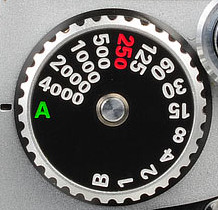
\includegraphics[scale=0.66]{log/nikon.jpg}
\caption{Shutter speed ($\frac{1}{x}$ of second) knob on photo camera}
\end{figure}

Another logarithmic scale familiar to anyone is decibel.
Even on cheap mp3 players and smartphones, where the volume is measured in conventional percents, this scale is logarithmic, 
and the difference between 50\% and 60\% may be much larger in sound pressure terms.

Yet another familiar to anyone logarithmic scale is Richter magnitude scale
\footnote{\url{https://en.wikipedia.org/wiki/Richter_magnitude_scale}}.
The Richter scale is practical, because when people talk about earthquakes, they are not interesting in exact scientific values
(in Joules or TNT equivalent), they are interesting in how bad damage is.

\myheading{In electronics engineering}

The loudspeakers are not perfect, so its output is non-linear in relation to input frequency.
In other word, loudspeaker has different loudness at different frequency.
It can be measured easily, and here is an example of plot of some speaker, I took it there:
\url{http://www.3dnews.ru/270838/page-3.html}.

\begin{figure}[H]
\centering
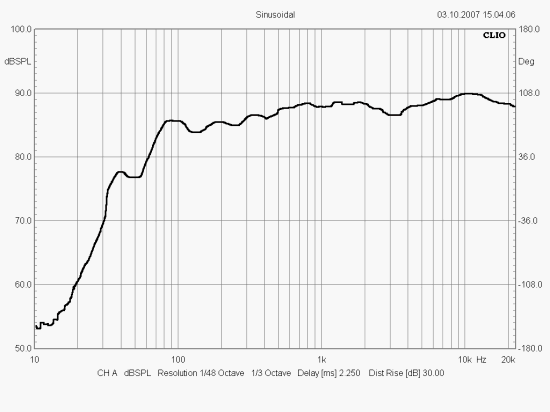
\includegraphics[scale=0.66]{log/65366.png}
\caption{Frequency response (also known as \textit{Bode plot}) of some loudspeaker}
\end{figure}

Both axis on this plot are logarithmic: y axis is loudness in decibel and x axis is frequency in Hertz.
Needless to say, the typical loudspeaker has bass/medium speaker + tweeter (high frequency speaker).
Some of more advanced loudspeaker has 3 speakers: bass, medium and tweeter.
Or even more.
And since the plot is logarithmic, each of these 2 or 3 speakers has their own part of plot, and these parts has comparable size.
If the x axis would be linear instead of logarithmic, the main part of it would be occupied by frequency response of tweeter alone, 
because it has widest frequency range. While bass speaker has narrowest frequency range, it would have very thin part of the plot.

y axis (vertical) of the plot is also logarithmic (its value is shown in decibels).
If this axis would be linear, the main part of it would be occupied by very loud levels of sound, while there would be thinnest line at the bottom
reserved for normal and quiet level of sounds.

Both of that would make plot unusable and impractical.
So both axis has logarithmic scale.
In strict mathematics terms, the plot shown is called \textit{log-log plot}, which means that both axis has logarithmic scale.

Summarizing, both electronics engineers and HiFi audio enthusiasts use these plots to compare quality of speakers.
These plots are often used in loudspeakers reviews
\footnote{Some of speakers of USSR era (like Latvian Radiotehnika S-30 and S-90) 
had such plots right on the surface of speaker box, presumably, for marketing purposes.}.

\myheading{In IT}

git, like any other VCS, can show a graph, how many changes each file got in each commit, for example:

\lstinputlisting{log/git_log.txt}

This scale is not logarithmical (I had a look into git internals), but this is exact place where logarithmical scale can be used.
When software developer got such report, he/she don't interesting in exact numbers of lines changed/added/removed.
He/she wants to see an outlook: which files got most changes/additions/removals, and which got less.

There is also a constraint: the space on the terminal is limited, so it's not possible to draw a minus or plus sign for each changed line of code.

Another example is Bitcoin client ``signal reception strength'', apparently, modeled after mobile phone signal indicator:

\begin{figure}[H]
\centering

\includegraphics[scale=1]{log/bitcoin_bars.png}
\caption{Bitcoin client}
\end{figure}

These bars indicating, how many connections client currently has.
Let's imagine, client can support up to 1000 connections, but user is never interesting in precise number, all he/she wants to know is how good its link
with Bitcoin network is.
I don't know how Bitcoin calculates this, but I think one bar could indicate that client has only 1 connection, two bars --- 2-5, three bars --- up to 10-20,
and four bars --- anything bigger.
This is also logarithmic scale.
On contrary, if you divide 1000 by 4 even parts, and one bar will fired if you've got 250 connections, two bars if you've got 500, etc, 
this would make the indicator useless, such indicators are no better than simple ``on/off'' lamp.

\myheading{Web 2.0}

Sites like GitHub, Reddit, Twitter sometimes shows how long some event was ago, instead of precise date (at least in 2015).
For example, Reddit may show date as ``3 years ago'', ``11 months ago'', ``3 weeks ago'', ``1 day ago'', ``10 hours ago'', etc, down to minutes and seconds.
You wouldn't see ``3 years and 11 hours ago''.
This is also logarithmic scale.
When some event happens 10 months ago, users are typically not interesting in precision down to days and hours.
When something happens 2 years ago, users usually not interesting in number of months and days in addition to these 2 years.

\levelup{}


\section{Multiplication and division using addition and subtraction}

It is possible to use addition instead of multiplication, using the following rule:

\begin{equation} \label{eq:1}
\log_{base} (ab) = \log_{base} (a) + \log_{base}(b)
\end{equation}

\dots while base can be any number.

It's like summing number of zeroes of two numbers. Let's say, you need to multiply 100 by 1000. Just sum number of their zeroes (2 and 3).
The result if the number with 5 zeroes. It's the same as $\log_{10} (100) + \log_{10} (1000) = \log_{10} (100000)$.

Division can be replaced with subtraction in the very same way.

\subsection{Logarithmic slide rule}

Here is very typical slide rule\footnote{I took screenshots at \url{http://museum.syssrc.com/static/sliderule.html}}.
It has many scales, but take a look on C and D scales, they are the same:

\begin{figure}[H]
\centering
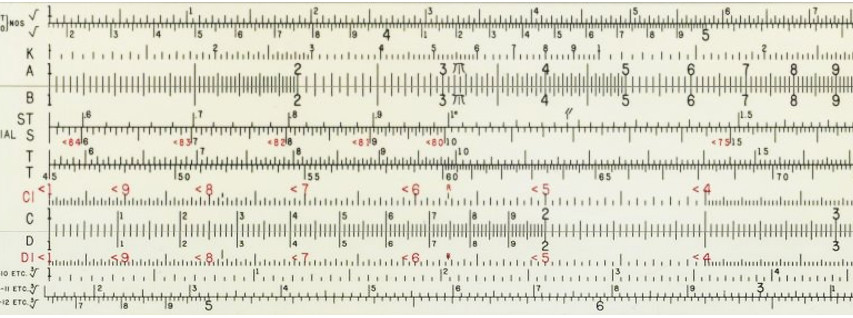
\includegraphics[scale=0.66]{log/sliderule1.jpg}
\caption{Initial state of slide rule}
\end{figure}

Now shift the core of rule so C scale at 1 will point to 1.2 at D scale:

\begin{figure}[H]
\centering
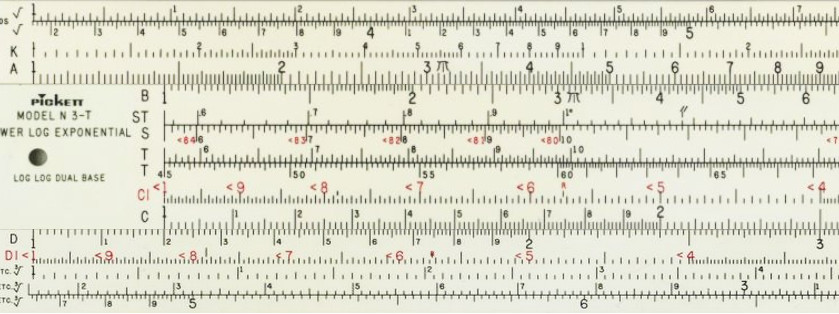
\includegraphics[scale=0.66]{log/sliderule2.jpg}
\caption{C scale shifted}
\end{figure}

% TODO дорисовать стрелки как в https://commons.wikimedia.org/wiki/File:Slide_rule_example2_with_labels.svg?uselang=ru

Find 2 at C scale and find corresponding value at D scale (which is 2.4).
Indeed, $1.2 \cdot 2 = 2.4$.
It works because by sliding scales we actually add distance between 1 and 1.2 (at any scale) to the distance between 1 and 2 (at any scale).
But since these scales logarithmic, addition of logarithmic values is the same as multiplication.

Values on scales can be interpreted as values of other order of magnitude.
We can say that 1 at C scale is actually point to 12 at D scale.
Find 1.8 at D scale (which is 18 now), it points somewhere between 21 and 22.
It's close: $12 \cdot 18 = 216$.

It works because of equation \ref{eq:1}.

Here is another example from Wikipedia:

\begin{figure}[H]
\centering
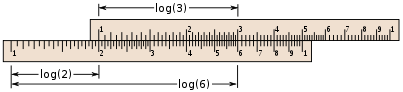
\includegraphics[scale=0.66]{log/403px-Slide_rule_example2_with_labels.svg.png}
\caption{Example from Wikipedia}
\end{figure}

\subsection{Logarithmic tables}

As we can see, the precision of logarithmic slide rule is up to 1 or 2 decimal digits after point.
Using precomputed logarithmic tables, it's possible to calculate product of two numbers with a precision up to $\approx 4$ digits.

First, find common (base of 10) logarithms of each number using logarithmic table:

\begin{figure}[H]
\centering
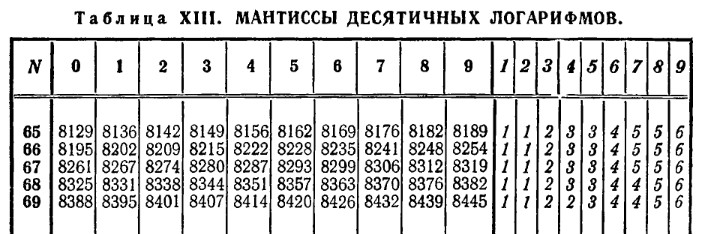
\includegraphics[scale=0.66]{log/bradis1.jpg}
\caption{Logarithmic tables}
\end{figure}

Then add these numbers. Find the number you got in table of powers of 10 ($10^{x}$, also called ``anti-log table''):

\begin{figure}[H]
\centering
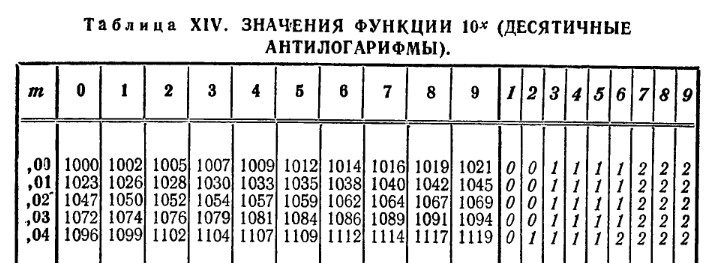
\includegraphics[scale=0.66]{log/bradis2.jpg}
\caption{Antilog tables}
\end{figure}

% TODO CRC book! спросить у него? http://www.mathtable.com/smtf/

Resulting number is a product.
The whole process may be faster than to multiply using long multiplication method using paper-n-pencil taught in schools.

Screenshots I took from the Bradis' book, once popular in USSR.
Another well-known book in western world with logarithmic and other tables is 
Daniel Zwillinger - CRC Standard Mathematical Tables and Formulae 
(up to 30th edition, the logarithmic tables are dropped after).

\subsection{Working with very small and very large numbers}

It's hard to believe, but the rule used on logarithmic slide rule for multiplication is still used sometimes in software code.
It's a problem to work with very small (denormalized) numbers
\footnote{Denormalized numbers in double-precision floating point format are numbers between $\approx 10^{324}$ and $\approx 10^{308}$} encoded in IEEE 754 standard. 

Here is my attempt to calculate $\frac{1.234 \times 10^{-300} \cdot 2.345678901234 \times 10^{-24}}{3.456789 \times 10^{-50}}$:

\begin{lstlisting}[caption=C code]
#include <stdio.h>
#include <math.h>

int main()
{
	double a=1.234e-300;
	double b=2.345678901234e-24;
	double c=3.456789e-50;
	printf ("%.30e\n", a*b/c);
};
\end{lstlisting}

The output is $1.429261797122261460966983388190 \times 10^{-274}$, which is incorrect.
When using debugger, we can see that the multiplication operation raises \textit{inexact exception} and \textit{underflow exception} in FPU.
The division operation also raises \textit{inexact exception}.

Let's check in Wolfram Mathematica:

\begin{lstlisting}[caption=Wolfram Mathematica]
In[]:= a = 1.234*10^(-300);

In[]:= b = 2.345678901234*10^(-24);

In[]:= c = 3.456789*10^(-50);

In[]:= a*b/c
Out[]= 8.37357*10^-275
\end{lstlisting}

The underflow exception raised in my C program because result of multiplication is in fact 
$2.894567764122756*10^{-324}$, which is even smaller than smallest denormalized number FPU can work with.

Let's rework our example to compute it all using natural logarithms 
(\texttt{exp(x)} is a C standard function, which computes $e^x$ and \texttt{log(x)} here is $\log_e(x)$ (or $ln(x)$)):

\begin{lstlisting}[caption=C code]
#include <stdio.h>
#include <math.h>

int main()
{
	double a=1.234e-300;
	double b=2.345678901234e-24;
	double c=3.456789e-50;
	printf ("%.30e\n", exp(log(a)+log(b)-log(c)));
};
\end{lstlisting}

Now the output is $8.373573753338710216281125792150 \times 10^{-275}$, same as Mathematica reported.

The same problem with very large numbers.

\begin{lstlisting}[caption=C code]
#include <stdio.h>
#include <math.h>

int main()
{
	double a=1.234e+300;
	double b=2.345678901234e+24;
	double c=3.456789e+50;
	printf ("%.30e\n", a*b/c);
};
\end{lstlisting}

When this program running, its result is ``inf'', meaning $\infty$, i.e., overflow occurred.
When using debugger, we can see than the multiplication operation raises \textit{inexact exception} plus \textit{overflow exception}.
The correct value in Wolfram Mathematica is...

\begin{lstlisting}[caption=Wolfram Mathematica]
In[]:= a = 1.234*10^300;

In[]:= b = 2.345678901234*10^24;

In[]:= c = 3.456789*10^50;

In[]:= a*b/c
Out[]= 8.37357*10^273
\end{lstlisting}

Let's rewrite our C example:

\begin{lstlisting}[caption=C code]
int main()
{
	double a=1.234e+300;
	double b=2.345678901234e+24;
	double c=3.456789e+50;
	printf ("%.30e\n", exp(log(a)+log(b)-log(c)));
};
\end{lstlisting}

Now the program reports $8.373573753337712538419923350878 \times 10^{273}$, which is correct value.

The way of representing all numbers as their logarithms called ``logarithmic number system''
\footnote{\url{https://en.wikipedia.org/wiki/Logarithmic_number_system}}.
It allows to work with numbers orders of magnitude lower than FPU can handle.

So why all computations are not performed using logarithms, if it's so good?
It's better only for very small or very large numbers.
Working with small and medium numbers, precision of its logarithmic versions will be much more important and harder to control.

Also, finding logarithm of a number with the following exponentiation are operations may be slower than multiplication itself.

\subsection{IEEE 754: adding and subtracting exponents}

IEEE 754 floating point number consists of sign, significand and exponent.
Internally, its simplified representation is:

\begin{equation}
(-1)^{sign} \cdot significand \times 2^{exponent}
\end{equation}

Given that, the FPU may process significands and exponents separately during multiplication, 
but when it processes exponents of two numbers, they are just summed up.
For example:

\begin{equation}
significand_{1} \times 2^{10} \cdot significand_{2} \times 2^{50} = significand_{3} \times 2^{60}
\end{equation}

\dots precise values of significands are omitted, but we can be sure, if the first number has exponent of $10$, the second has $50$,
the exponent of the resulting number will be $\approx 60$.

Conversely, during division, exponent of divisor is subtracted from the exponent of the dividend.

\begin{equation}
\frac{significand_{1} \times 2^{10}}{significand_{2} \times 2^{50}} = significand_{3} \times 2^{-40}
\end{equation}

I don't have access to Intel or AMD FPU internals, but I can peek into OpenWatcom FPU emulator libraries
\footnote{It was a time in 1980s and 1990s, when FPU was expensive and it could be bought separately 
in form of additional chip and added to x86 computer.
And if you had run a program which uses FPU on the computer where it's missing, FPU emulating library might be an option.
Much slower, but better than nothing.}.

Here is summing of exponents during multiplication:\\
\url{https://github.com/open-watcom/open-watcom-v2/blob/86dbaf24bf7f6a5c270f5a6a50925f468d8d292b/bld/fpuemu/386/asm/fldm386.asm\#L212}.\\
And here is subtracting of exponents during division:\\
\url{https://github.com/open-watcom/open-watcom-v2/blob/e649f6ed488eeebbc7ba9aeed8193d893288d398/bld/fpuemu/386/asm/fldd386.asm\#L237}.

Here is also multiplication function from FPU emulator in Linux kernel:
\url{https://github.com/torvalds/linux/blob/da957e111bb0c189a4a3bf8a00caaecb59ed94ca/arch/x86/math-emu/reg_u_mul.S\#L93}.

\subsection{Check, if the product will overflow}

Using logarithmic versions of two numbers, it is easy to check if the product of them will overflow in current environment (32-bit or 64-bit CPU registers).
Perhaps, programming languages with dynamic typing (like LISP, Python, Ruby, BASIC, etc) can check, 
if the current number must be switched to bignum (if the result is too big to fit in the CPU register) or not.



\myheading{Exponentiation}

Using equation \ref{eq:1} we may quickly notice that

\begin{equation}
b^n = \underbrace{b \times \cdots \times b}_n = base^{(\log_{base} (b))*n}
\end{equation}

That works with any logarithmic base.
In fact, this is the way how exponentiation is computed on computer.
x86 CPU and x87 FPU has no special instruction for it.

This is the way how pow() function works in Glibc: \url{https://github.com/lattera/glibc/blob/master/sysdeps/x86_64/fpu/e_powl.S\#L189}:\\

\begin{lstlisting}[caption={Glibc source code, fragment of the pow() function}]

...

7:	fyl2x			// log2(x) : y
8:	fmul	%st(1)		// y*log2(x) : y
	fst	%st(1)		// y*log2(x) : y*log2(x)
	frndint			// int(y*log2(x)) : y*log2(x)
	fsubr	%st, %st(1)	// int(y*log2(x)) : fract(y*log2(x))
	fxch			// fract(y*log2(x)) : int(y*log2(x))
	f2xm1			// 2^fract(y*log2(x))-1 : int(y*log2(x))
	faddl	MO(one)		// 2^fract(y*log2(x)) : int(y*log2(x))
	fscale			// 2^fract(y*log2(x))*2^int(y*log2(x)) : int(y*log2(x))
	fstp	%st(1)		// 2^fract(y*log2(x))*2^int(y*log2(x))

...

\end{lstlisting}

x87 FPU has the following instructions used Glibc's version of pow() function:
FYL2X (compute $y \cdot log_2 x$), F2XM1 (compute $2^x–1$).
Even more than that, FYL2X instruction doesn't compute binary logarithm alone, it also performs multiplication operation, 
to provide more easiness in exponentiation computation.

It works because calculating $2^x$ (exponentiation with base 2) is faster than exponentiation of arbitrary number.

Using hacker's tricks, it's also possible to take advantage of the IEEE 754 format and SSE instructions set:\\
\url{http://stackoverflow.com/a/6486630/4540328}.


\myheading{Square root}

Likewise, square root can be computed in the following way:

\begin{equation}
\sqrt[2]{x} = 2^{\frac{\log_2{x}}{2}}
\end{equation}

This leads to an interesting consequence: if you have a value stored in logarithmical form and you need to take
square root of it and leave it in logarithmical form, all you need is just to divide it by 2.

And since floating point numbers encoded in IEEE 754 has exponent encoded in logarithmical form,
you need just to shift it right by 1 bit to get square root:
\url{https://en.wikipedia.org/wiki/Methods_of_computing_square_roots#Approximations_that_depend_on_the_floating_point_representation}.

Likewise, cube root and nth root can be calculated using logarithm of corresponding base:

\begin{equation}
\sqrt[b]{x} = b^{\frac{\log_b{x}}{b}}
\end{equation}


\section{Base conversion}

FYL2X and F2XM1 instructions are the only logarithm-related x87 FPU has.
Nevertheless, it's possible to compute logarithm with any other base, using these.
The very important property of logarithms is:

\begin{equation}
\log_y (x) = \frac{\log_a (x)}{\log_a (y)}
\end{equation}

So, to compute common (base 10) logarithm using available x87 FPU instructions, we may use this equation:

\begin{equation}
\log_{10} (x) = \frac{\log_2 (x)}{\log_2 (10)}
\end{equation}

\dots while $\log_2(10)$ can be precomputed ahead of time.

Perhaps, this is the very reason, why x87 FPU has the following instructions:
FLDL2T (load $\log_2 (10)=3.32193...$ constant) and FLDL2E (load $\log_2 (e)=1.4427...$ constant).

Even more than that.
Another important property of logarithms is:

\begin{equation}
\log_y (x) = \frac{1}{\log_x (y)}
\end{equation}

Knowing that, and the fact that x87 FPU has FYL2X instruction (compute $y \cdot log_2 x$), logarithm base conversion can be done using multiplication:

\begin{equation}
\log_y (x) = \log_a (x) \cdot \log_y (a)
\end{equation}

So, computing common (base 10) logarithm on x87 FPU is:

\begin{equation}
\log_{10} (x) = \log_2 (x) \cdot \log_{10} (2)
\end{equation}

Apparently, that is why x87 FPU has another pair of instructions:

FLDLG2 (load $\log_{10} (2)=0.30103...$ constant) and FLDLN2 (load $\log_e (2)=0.693147...$ constant).

Now the task of computing common logarithm can be solved using just two FPU instructions: FYL2X and FLDLG2.

This piece of code I found inside of Windows NT4 ( \texttt{src/OS/nt4/private/fp32/tran/i386/87tran.asm} ), 
this function is capable of computing both common and natural logarithms: 

\begin{lstlisting}[caption=Assembly language code]
lab fFLOGm
        fldlg2                          ; main LOG10 entry point
        jmp     short fFYL2Xm

lab fFLNm                               ; main LN entry point
        fldln2

lab fFYL2Xm
        fxch
        or      cl, cl                  ; if arg is negative
        JSNZ    Yl2XArgNegative         ;    return a NAN
        fyl2x                           ; compute y*log2(x)
        ret
\end{lstlisting}



\myheading{Binary logarithm}

Sometimes denoted as lb(), binary logarithms are prominent in computer science, 
because numbers are usually stored and processed in computer in binary form.

\leveldown{}

\myheading{Denoting a number of bits for some value}

How many bits we need to allocate to store googol number ($10^{100}$)?

\begin{lstlisting}[caption=Wolfram Mathematica]
In[]:= Log2[10^100] // N
Out[]= 332.193
\end{lstlisting}

Binary logarithm of some number is the number of how many bits needs to be allocated.

If you have a variable which always has $2^x$ form, it's a good idea to store a binary logarithmic representation ($\log_2 (x)$) instead of it.
There are at least two reasons:
1) the programmer shows to everyone that the number has always $2^x$ form;
2) it's error-prone, it's not possible to accidentally store a number in some other form to this variable, so this is some kind of protection;
3) logarithmic representation is more compact.
There is, however, performance issue: the number must be converted back, but this is just one shifting operation (\texttt{1<<log\_n}).

Here is an example from NetBSD NTP client ( \texttt{netbsd-5.1.2/usr/src/dist/ntp/include/ntp.h} ):

\begin{lstlisting}[caption=C code]
/*
 * Poll interval parameters
 */
...
#define NTP_MINPOLL     4       /* log2 min poll interval (16 s) */
#define NTP_MINDPOLL    6       /* log2 default min poll (64 s) */
#define NTP_MAXDPOLL    10      /* log2 default max poll (~17 m) */
#define NTP_MAXPOLL     17      /* log2 max poll interval (~36 h) */
\end{lstlisting}

Couple examples from zlib (\texttt{deflate.h}):

\begin{lstlisting}[caption=C code]
    uInt  w_size;        /* LZ77 window size (32K by default) */
    uInt  w_bits;        /* log2(w_size)  (8..16) */
    uInt  w_mask;        /* w_size - 1 */
\end{lstlisting}

Another piece from zlib ( \texttt{contrib/blast/blast.c} ):

\begin{lstlisting}[caption=C code]
    int dict;           /* log2(dictionary size) - 6 */
\end{lstlisting}

If you need to generate bitmasks in range 1, 2, 4, 8...0x80000000, it is good idea to assign self-documenting name to iterator variable:

\begin{lstlisting}[caption=C code]
for (log2_n=1; log2_n<32; log2_n++)
    1<<log2_n;
\end{lstlisting}

Now about compactness, here is the fragment I found in OpenBSD, related to SGI IP22 architecture
\footnote{\url{http://www.linux-mips.org/wiki/IP22}} \\
( \texttt{OS/OpenBSD/sys/arch/sgi/sgi/ip22\_machdep.c} ):

\begin{lstlisting}[caption=C code]
                /*
                 * Secondary cache information is encoded as WWLLSSSS, where
                 * WW is the number of ways
                 *   (should be 01)
                 * LL is Log2(line size)
                 *   (should be 04 or 05 for IP20/IP22/IP24, 07 for IP26)
                 * SS is Log2(cache size in 4KB units)
                 *   (should be between 0007 and 0009)
                 */
\end{lstlisting}

Here is another example of using binary logarithm in Mozilla JavaScript engine (JIT compiler)
\footnote{\url{http://fossies.org/linux/seamonkey/mozilla/js/src/jit/mips/CodeGenerator-mips.cpp}}.
If some number is multiplied by $2^x$, the whole operation can be replaced by bit shift left.
The following code ( \texttt{js/src/jit/mips/CodeGenerator-mips.cpp} ), 
when translating multiplication operation into MIPS machine code, first, get assured if the number 
is really has $2^x$ form, then it takes binary logarithm of it and generates MIPS SLL instruction, which states for ``Shift Left Logical''.

\begin{lstlisting}[caption=Mozilla JavaScript JIT compiler (translating multiplication operation into MIPS bit shift instruction)]
bool
 CodeGeneratorMIPS::visitMulI(LMulI *ins)
 {
           default:
             uint32_t shift = FloorLog2(constant);
 
             if (!mul->canOverflow() && (constant > 0)) {
                 // If it cannot overflow, we can do lots of optimizations.
                 uint32_t rest = constant - (1 << shift);
 
                 // See if the constant has one bit set, meaning it can be
                 // encoded as a bitshift.
                 if ((1 << shift) == constant) {
                     masm.ma_sll(dest, src, Imm32(shift));
                     return true;
                 }

...

\end{lstlisting}

Thus, for example, $x=y \cdot 1024$ (which is the same as $x=y \cdot 2^{10}$) translates into $x=y<<10$.

\myheading{Calculating binary logarithm}

If all you need is integer result of binary logarithm ($abs(\log_2(x))$ or $\lfloor \log_2(x) \rfloor$), 
calculating is just counting all binary digits in the number minus 1.
In practice, this is the task of calculating leading zeroes.

Here is example from Mozilla libraries ( \texttt{mfbt/MathAlgorithms.h}
\footnote{\url{http://fossies.org/linux/seamonkey/mozilla/mfbt/MathAlgorithms.h}} ):

\begin{lstlisting}[caption=Mozilla libraries]
class FloorLog2<T, 4>
{
public:
   static uint_fast8_t compute(const T aValue)
   {
     return 31u - CountLeadingZeroes32(aValue | 1);
   }
 };

inline uint_fast8_t
 CountLeadingZeroes32(uint32_t aValue)
 {
   return __builtin_clz(aValue);
 }
\end{lstlisting}

Latest x86 CPUs has LZCNT (Leading Zeroes CouNT) instruction for that
\footnote{GNU \texttt{\_\_builtin\_clz()} function on x86 architecture can be thunk for LZCNT}, 
but there is also BSR (Bit Scan Reverse) instruction appeared in 80386, which can be used for the same purpose.
More information about this instruction on various architectures: \url{https://en.wikipedia.org/wiki/Find_first_set}.

There are also quite esoteric methods to count leading zeroes without this specialized instruction: \url{http://yurichev.com/blog/de_bruijn/}.

\myheading{O(log n) time complexity}

Time complexity\footnote{\url{https://en.wikipedia.org/wiki/Time_complexity}} is a measure of speed of a specific algorithm 
in relation to the size of input data.

O(1) -- time is always constant, to matter what size of input data. Simplest example is object getter -- it just returns some value.

O(n) -- time is linear, growing according to the size of input data. Simplest example is search for some value in the input array.
The larger array, the slowest search.

O(log n) -- time is logarithmic to the input data.
Let's see how this can be.

Let's recall child's number guessting game\footnote{\url{http://rosettacode.org/wiki/Guess_the_number}}.
One player think about some number, the other should guess it, offering various versions.
First player answers, is guessed number is larger or less.
Typical dialogue can be as the follows:

\begin{lstlisting}
-- I think of a number in 1..100 range.
-- Is it 50?
-- My number is larger.
-- 75?
-- It is lesser.
-- 63?
-- Larger.
-- 69?
-- Larger.
-- 72?
-- Lesser.
-- 71?
-- Correct.
\end{lstlisting}

Best possible strategy is to divide the range in halves.
The range is shorten at each step by half.
At the very end, the range has lenght of 1, and this is correct answer.
Maximal number of steps using the strategy described here are $\log_2(initial\_range)$.
In our example, initial range is 100, so the maximum number of steps is 6.64... or just 7.
If the initial range is 200, maximum number of steps are $\log_2(200)=7.6..$ or just 8. The number of steps increasing by 1 when the range is doubled.
Indeed, doubled range indicates that the guesser needs just one more step at the start, not more.
If the initial range is 1000, numbers of steps are $\log_2(1000)=9.96...$ or just 10.

This is exactly O(log n) time complexity.\\
\\
Now let's consider couple of practical real-world algorithms.
One interesting thing is that if the input array is sorted, and its size is known, and we need to find some value in it, the algorithm works exactly
in the same way as child's number guessing game!
The algorithm starts in the middle of array and compare the value there with the value sought-after.
Depending on the result (larger or lesser), the \textit{cursor} is moved left or right and operating range is decreasing by half.
This is called binary search\footnote{\url{https://en.wikipedia.org/wiki/Binary_search_algorithm}}, and there is the \texttt{bsearch()} function in 
standard C/C++ library\footnote{\url{http://en.cppreference.com/w/cpp/algorithm/bsearch}}.\\
\\
Here is how binary search is used in git: \url{https://www.kernel.org/pub/software/scm/git/docs/git-bisect.html}.\\
\\
Another prominent example in CS is binary trees. They are heavily used internally in almost any programming language, when you use set, map, dictionary, etc.

Here is a simple example with the following numbers (or keys) inserted into binary tree:
0, 1, 2, 3, 5, 6, 9, 10, 11, 12, 20, 99, 100, 101, 107, 1001, 1010.

\tikzset
{
  treenode/.style = {align=center, inner sep=0pt, text centered},
  key/.style = {treenode, circle, white, draw=black, fill=black, minimum size=2.0em, text width=2.0em},
  empty/.style = {treenode, rectangle, draw=black, minimum width=0.5em, minimum height=0.5em}
}

\begin{center}
\begin{tikzpicture}[->,>=stealth',
		level 1/.style={sibling distance=6cm},
		level 2/.style={sibling distance=2.7cm},
		level 3/.style={sibling distance=1.7cm},
		level 4/.style={sibling distance=0.7cm}] 
	\node [key] {10}
	child { node [key] {1} 
		child{ node [key] {0} 
		}
		child{ node [key] {5}
			child{ node [key] {3}
				child{ node[key] {2}}
				child{ node[empty] {}}
			}
			child{ node [key] {6}
				child{ node[empty] {}}
				child{ node[key] {9}}
			}
		}                            
	}
	child { node [key] {100}
		child { node [key] {20}
			child{ node [key] {12}
				child{ node[key] {11}}
				child{ node[empty] {}}
			}
			child{ node [key] {99}
			}
		}
		child{ node [key] {107}
			child{ node [key] {101}}
			child{ node [key] {1001}
				child{ node[empty] {}}
				child{ node[key] {1010}}
			}
		}
	}
	; 
\end{tikzpicture}
\end{center}


And here is how binary tree search works: put \textit{cursor} at the root. Now compare the value under it with the value sought-after.
If the value we are seeking for is lesser than the current, take a move into left node. If it's bigger, move to the right node.
Hence, each left descendant node has value lesser than in 
ascendant node.
Each right node has value which is bigger.
The tree must be rebalanced after each modification (I gave examples of it in my book about reverse engineering (\url{http://beginners.re/}, 51.4.4)).
Nevertheless, lookup function is very simple, and maximal number of steps is $\log_n(number\_of\_nodes)$.
We've got 17 elements in the tree at the picture, $\log_2(17)=4.08...$, indeed, there are 5 tiers in the tree.

\levelup{}


\section{Common (base 10) logarithms}

Also known as ``decimal logarithms''.
Denoted as \texttt{lg} on handheld calculators.

10 is a number inherently linked with human's culture, since almost all humans has 10 digits.
Decimal system is a result of it.
Nevertheless, 10 has no special meaning in mathematics and science in general.
So are common logarithms.

One notable use is a decibel logarithmic scale, which is based of common logarithm.

Common logarithms are sometimes used to calculate space for decimal number in the string or on the screen.
How many characters you should allocate for 64-bit number? 20, because $log_{10}(2^{64}) = 19.2...$.

Functions like \texttt{itoa()}\footnote{\url{http://www.cplusplus.com/reference/cstdlib/itoa/}}
(which converts input number to a string) can calculate output buffer size precisely, 
calculating common logarithm of the input number.


\myheading{Natural logarithm}

Natural logarith (denoted as \texttt{ln} on handheld calculators, and sometimes denoted just as \texttt{log})
is logarithm of base $e=2.718281828...$.
Where this constant came from?

\leveldown{}

\myheading{Savings account in your bank}

Let's say you make a deposit into bank, say, 100 dollars (or any other currency).
They offer 2.5\% per year (annual percentage yield).
This mean, you'll can get doubled amount of money (200 dollars) after 40 years.
So far so good.
But some banks offers compound interest.
Also called ``complex percent'' in Russian language, where ``complex'' in this phrase is closer to the word ``folded''.
This mean, after each year, they pretend you withdraw your money with interest, then redeposit them instantly.
Banks also say that the interest is recapitalized once a year.
Let's calculate final amount of money after 40 years:

\lstinputlisting[caption=Python code]{log/APY1.py}

\begin{lstlisting}
year= 0 amount at the end 102.5
year= 1 amount at the end 105.0625
year= 2 amount at the end 107.6890625
year= 3 amount at the end 110.381289063
...
year= 36 amount at the end 249.334869861
year= 37 amount at the end 255.568241608
year= 38 amount at the end 261.957447648
year= 39 amount at the end 268.506383839
\end{lstlisting}

The thing is that the final amount (268.50...) is aimed toward $e$ constant.

Now there is another bank, which offers to recapitalize your deposit each month.
We'll rewrite our script slightly:

\lstinputlisting[caption=Python code]{log/APY2.py}

\begin{lstlisting}
year= 0 month= 0 amount 100.208333333
year= 0 month= 1 amount 100.417100694
year= 0 month= 2 amount 100.626302988
year= 0 month= 3 amount 100.835941119
...
year= 39 month= 8 amount 269.855455383
year= 39 month= 9 amount 270.417654248
year= 39 month= 10 amount 270.981024361
year= 39 month= 11 amount 271.545568162
\end{lstlisting}

The final result is even closer to $e$ constant.

Let's imagine there is a bank which allows to recapitalize each day:

\lstinputlisting[caption=Python code]{log/APY3.py}

\begin{lstlisting}
year= 0 month= 0 day= 0 amount 100.006944444
year= 0 month= 0 day= 1 amount 100.013889371
year= 0 month= 0 day= 2 amount 100.02083478
year= 0 month= 0 day= 3 amount 100.027780671
...
year= 39 month= 11 day= 26 amount 271.762123927
year= 39 month= 11 day= 27 amount 271.780996297
year= 39 month= 11 day= 28 amount 271.799869977
year= 39 month= 11 day= 29 amount 271.818744968
\end{lstlisting}

The final amount of money is more closer to $e$ constant.

If to imagine some really crazy bank client who redeposit his deposit infinite number of times per each day, the final value after 40 years
would be $100 \cdot e$.
It's not possible in the real world, so the final amount is approaches this value, but is never equal to it.
Mathematically speaking, its limit is $100 \cdot e$.

\myheading{Exponential decay}

\leveldown{}

\myheading{Capacitor discharge}

% TODO redraw! ибо спизжено. https://en.wikipedia.org/wiki/Talk%3ARC_circuit#RC_Circuits
\begin{figure}[H]
\centering
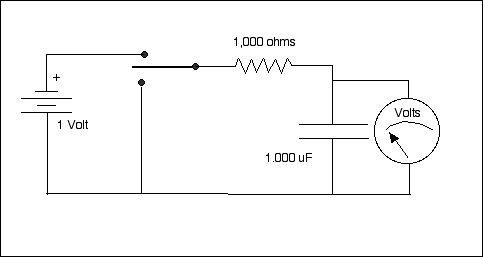
\includegraphics[scale=0.66]{log/Schematic_of_Battery_and_Capacitor.jpg}
\end{figure}

From electronics engineering course we may know that the capacitor discharging by half after $RC\ln(2)$ seconds,
where C is capacity of capacitor in farads and R resistance of resistor in ohms.
Given $1k\Omega$ resistor and $1000 \mu F$ capacitor, what its voltage after 1 seconds will be? after 2 seconds?
It's discharge can be calculated using this equation:

\LARGE\[
V=V_0 \cdot e^{\frac{-t}{RC}}
\]
\normalsize

\dots where $V_0$ is initial charge in volts, $t$ is time in seconds and $e$ is base of natural logarithm.

Let's see it in Wolfram Mathematica:

\begin{lstlisting}[caption=Wolfram Mathematica]
r = 1000; (* resistance in ohms *)

c = 0.001; (* capacity in farads *)

v = 1; (* initial voltage *)

Plot[v*E^((-t)/(r*c)), {t, 0, 5}, 
 GridLines -> {{Log[2], Log[2]*2, Log[2]*3}, {0.5, 0.25, 0.125}},
 Epilog -> {Text["ln(2)", {Log[2], 0.05}], 
   Text["ln(2)*2", {Log[2]*2, 0.05}], 
   Text["ln(2)*3", {Log[2]*3, 0.05}],
   Text["1/2", {0.1, 0.5}], Text["1/4", {0.1, 0.25}], 
   Text["1/8", {0.1, 0.128}]}, AxesLabel -> {seconds, voltage}]
\end{lstlisting}

\begin{figure}[H]
\centering
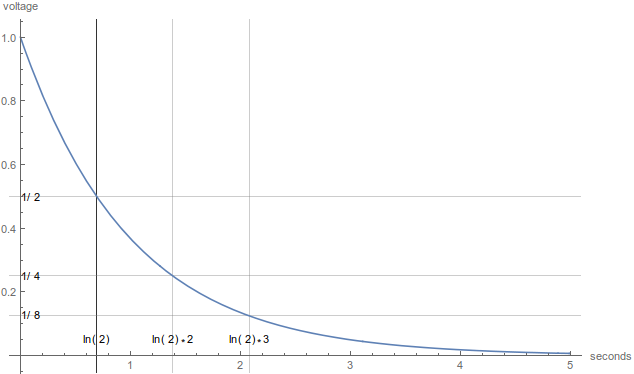
\includegraphics[scale=0.66]{log/capacitor_discharge.png}
\caption{Capacitor voltage during discharge}
\end{figure}

As we can see, $\frac{1}{2}$ of initial charge is left after $ln(2)$ seconds (~0.69...), 
and $\frac{1}{4}$ of charge is left after $ln(4)$ seconds (~1.38...).

Indeed, if we interesting in precise time in seconds, when charge will be $\frac{1}{x}$, just calculate $ln(x)$.

Now here is the same plot, but I added two more labels, $\frac{1}{3}$ and $\frac{1}{7}$:

\begin{lstlisting}[caption=Wolfram Mathematica]
Plot[v*E^((-t)/(r*c)), {t, 0, 5}, 
 GridLines -> {{Log[3], Log[7]}, {1/3, 1/7}},
 Epilog -> {Text["ln(3)", {Log[3], 0.05}], 
   Text["ln(7)", {Log[7], 0.05}],
   Text["1/3", {0.1, 1/3}], Text["1/7", {0.1, 1/7}]}, 
 AxesLabel -> {seconds, voltage}]
\end{lstlisting}

\begin{figure}[H]
\centering
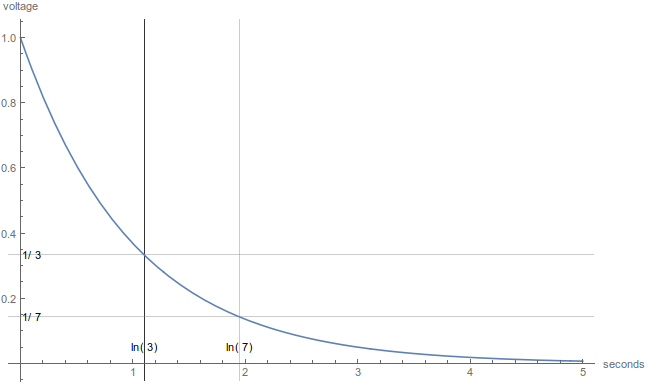
\includegraphics[scale=0.66]{log/capacitor_discharge2.png}
\caption{Capacitor voltage during discharge}
\end{figure}

\dots and we see that these points corresponds to $ln(3)$ and $ln(7)$.
That means, $\frac{1}{3}$ of charge is left after $ln(3) \approx 1.098...$ seconds and $\frac{1}{7}$ of charge after $ln(7) \approx 1.945...$ seconds.

\myheading{Radioactive decay}

Radioactive decay is also exponential decay.
Let's take Polonium 210 as an example\footnote{\url{https://en.wikipedia.org/wiki/Polonium}}.
It's half-life (calculated) is $\approx 138.376$ days.
That means that if you've got 1kg of Polonium 210, after $\approx 138$ days, half of it (0.5 kg) left as \textsuperscript{210}Po and 
another half is transformed into \textsuperscript{206}Pb (isotope of lead\footnote{\url{https://en.wikipedia.org/wiki/Isotopes_of_lead\#Lead-206}}).
After another $\approx 138$ days, you'll get $\frac{3}{4}$ of isotope of lead and $\frac{1}{4}$ will left as \textsuperscript{210}Po.
After another $\approx 138$ days, amount of Polonium will be halved yet another time, etc.

The equation of radioactive decay is:

\[
N=N_{0}e^{-\lambda t}
\]

\dots where $N$ is number of atoms at some point of time, $N_{0}$ is initial number of atoms, $t$ is time, $\lambda$ is decay constant.
Decay of Polonium is exponential, but decay constant is the constant, defining how fast (or slow) it will fall.

Here we go in Mathematica, let's get a plot for 1000 days:

\begin{lstlisting}[caption=Wolfram Mathematica]
l = 0.005009157516910051; (* decay constant of Polonium 210 *)

hl = Log[2]/l
138.376

Plot[E^(-l*t), {t, 0, 1000}, 
 GridLines -> {{hl, hl*2, hl*3}, {0.5, 0.25, 0.125}}, 
 Epilog -> {Text["hl", {hl, 0.05}], Text["hl*2", {hl*2, 0.05}], 
   Text["hl*3", {hl*3, 0.05}], Text["1/2", {30, 0.5}], 
   Text["1/4", {30, 0.25}], Text["1/8", {30, 0.128}]}, 
 AxesLabel -> {days, atoms}]
\end{lstlisting}

\begin{figure}[H]
\centering
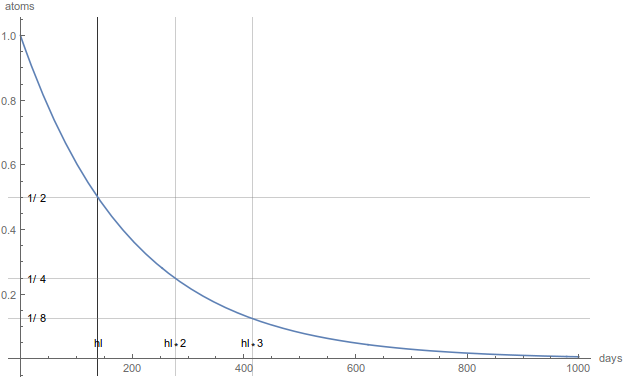
\includegraphics[scale=0.66]{log/210po.png}
\caption{Exponential decay of Polonium 210}
\end{figure}

\myheading{Beer froth}

There is even the paper (got Ig Nobel prize in 2002), author's of which demonstrates that beer froth is also decays exponentially:
\url{http://iopscience.iop.org/0143-0807/23/1/304/},
\url{https://classes.soe.ucsc.edu/math011a/Winter07/lecturenotes/beerdecay.pdf}.

\begin{figure}[H]
\centering
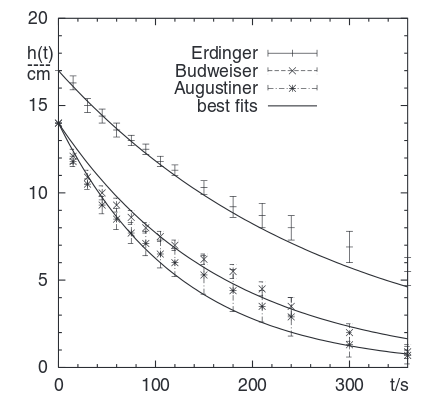
\includegraphics[scale=0.66]{log/beer.png}
\caption{Results from the paper}
\end{figure}

The paper can be taken as a joke, nevertheless, it's a good demonstration of exponential decay.

\myheading{Conclusion}

Capacitor discharge and radioactive decay obeys the same law of halving some amount after equal gaps of time:

\[
amount=amount_{0} \cdot e^{- decay\_constant \cdot time}
\]

Decay constant in case of capacitor discharge defined by product of resistance and capacity.
The bigger one of them, the slower decay.

Natural logarithm is used to calculate gap of time (half-life or half-time) judging by decay constant.

\levelup{}

\levelup{}


% TODO \section{Cheat sheet}

\levelup{}



\end{document}
